\section{Program Representation}
When translating a program to a UPPAAL of the program. Several representations are possible, depending on what one wants to show. One could for example represent a program merely in terms of program flow if a simulation of a disruption of the program flow is to be shown, e.g an error in the program counter. One could also include the data flow in the program if a simulation of a corruption of a memory value is to be shown. These are just a few examples and many representations can be chosen.\\

We have chosen the later and model the program in terms of program flow and data flow, so that we can simulation disruptions in the programs execution flow. 


\subsection{Representation Details}
The program simulation is based on \jcl semantics, most Java bytecodes can be translated directly to \jcl at the loss of type information.\\
\kri{what does it mean for us?}
When representing Java bytecode in UPPAAL we have chosen to represent an instruction, such as \texttt{aload a} and \texttt{dup}, as UPPAAL locations. 
This implies that a change in the program counter is a change of the location. 
In turn this means that when an instruction is to be executed the change to the program configuration \textit{Conf} from  \cref{sec:semintro} occurs on the edge to next location.

\begin{lstlisting}[caption=Jave code sample.]
public class Sample{
    public static void main(String[] args) {
        for (String a : args)         
        {
            System.out.print(a);
        }
    }
}
\end{lstlisting}

\begin{lstlisting}[caption=Bytecode sample.]
public static void main(java.lang.String[]);
 Code:
   0: aload_0       
   1: astore_1      
   2: aload_1       
   3: arraylength   
   4: istore_2      
   5: iconst_0      
   6: istore_3      
   7: iload_3       
   8: iload_2       
   9: if_icmpge     31
  12: aload_1       
  13: iload_3       
  14: aaload        
  15: astore        4
  17: getstatic     #2                  // Field java/lang/System.out:Ljava/io/PrintStream;
  20: aload         4
  22: invokevirtual #3                  // Method java/io/PrintStream.print:(Ljava/lang/String;)V
  25: iinc          3, 1
  28: goto          7
  31: return        

\end{lstlisting}

\begin{figure}[H]
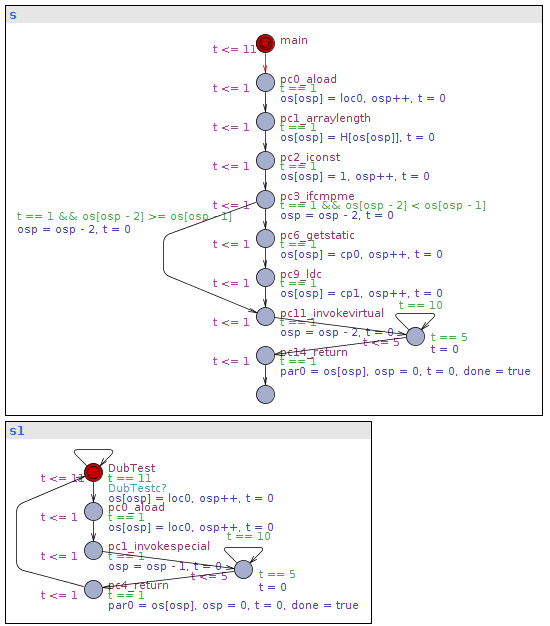
\includegraphics[width=\textwidth]{generated_wip}
\caption{Auto generated model, work in progress.}
\label{fig:generated_wip}
\end{figure}
\kri{update the model for the new sample}

\subsubsection{Simple Instructions}
\begin{figure}[H]
\centering
\begin{subfigure}{.3\textwidth}
  \begin{lstlisting}
  0. aload 0
  1. arraylength
  ...
  \end{lstlisting}
  \caption{Java Bytecode Sample.}
\end{subfigure} 
\hspace{10px}
\begin{subfigure}{.6\textwidth}
  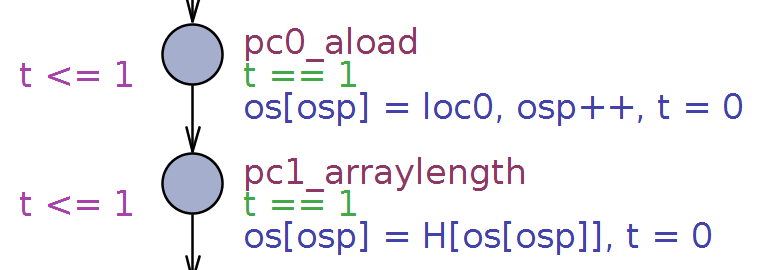
\includegraphics[width=\textwidth]{UPPAAL1.png}
  \caption{Generated model from Sample.}
\end{subfigure}
\caption{Java bytecode and corresponding UPPAAL model.}
\label{fig:uppaal1}
\end{figure}
\kri{lav ny model til nyt sample}
\Cref{fig:uppaal1} show how two Java Bytecode instructions are represented in UPPAAL. On the left we see the Java bytecode, the first line with program counter 0 we have the \texttt{aload 0} instruction. \texttt{aload 0} pushes a reference to the top of the operation stack from local variables at position zero, then increments the operand stack pointer and program counter.

%uppaal location edge
In UPPAAL the location \texttt{pc0\_aload} represent \texttt{aload 0}. The UPPAAL model is seen in \Cref{fig:uppaal1}b. We simulate execution time with the location invariant \texttt{t <= 1}  and guard \texttt{t == 1} on the edge leading to the next location. The guard is found right below the location name right of the edge and invariant is to the left of the edge. In this sample we defined the execution time as 1 time unit.

In the update on the edge seen below the guard, we simulate the data flow by assigning the value of the local variable \texttt{loc0} to the top of the operand stack \texttt{os} represented by operand stack pointer \texttt{osp}. \texttt{osp} is incremented as the operand stack grows, the increment of the program counter is simulated by the edge itself.

\subsubsection{Jumps and Branches}
For the majority of instructions the program counter is set to the next instruction after execution, but for a jump with \texttt{goto a} the edge goes to the instruction with the program counter corresponding with value of \texttt{a}.

Conditionals such as \texttt{if\_cmpeq a} is the only instruction that is modelled by a location having two outgoing edges , one to the next instruction and one for the program counter of a. On these edges the guard is used to determine which of the edges is to be traversed. \kri{insert example}
\subsubsection{Method Calls}\label{subsubsec:method}
Method calls are represented by three additions to the model. These additions consist of locations, but they do not have any associated program counter since they are not a part of the original program.\\

% special case for main
The first is an addition of a location in the template of the \texttt{main} method. This location captures the notion that this is the start of the program.\\

% caller
The second is a new location in the caller for every method call it performs. This makes it possible to simulate parameter passing, as well as control transfer when waiting for a callee to return control to the caller after a method call. The simulation of the caller remains in this location until the callee returns control, after its simulation has finished. This control transfer is modeled with a synchronisation on the edge going from the new state in the caller and back to its original control flow.\ch{insert ref to figure}~\\

% callee
The third is an addition of two additional states in every template, except for the \texttt{main} template. The first, initial, location serves dual purposes: it enables the control transfer from the caller to itself by synchronisation, and simulates passing of arguments into the method from the caller. The second location is the \textit{Done} location, where the simulation ends up when it has finished its simulation. This is where control is transferred back to the caller.
\ch{show how parameters are passed in figure}
\ch{rewrite this}
\section{Modelling a Fault Injection}
\ch{we should also show how we have modelled a fault in the heap/stack}
To simulate a single bit flip occurring in the program's execution a special fault template is introduced. The template calculates a random value between $0$ and the maximum possible global clock value, which represents when in the programs execution a fault happens. The random value is assigned to a global variable in the UPPAAL system.\\\\
Every instruction in the Java bytecode is represented by a location, and has an associated program counter. There are edges from each location going to the locations which can be reached if one bit is flipped in the program counter. These edges have guards which check whether the time the fault is injected, corresponds to the global clock at the time the model simulation is at that particular edge. If it is, the guard will allow the edge to be traversed. There are no fault edges going back to the added locations described in \cref{subsubsec:method}, since these are not a part of the original program and therefore do not have an associated program counter.
\begin{figure}[H]
\centering
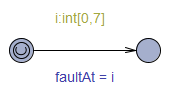
\includegraphics{figures/fault.PNG}
\caption{The UPPAAL template which performs a bit flip in the program counter}
\end{figure}\ch{update figure to use fault at between 0 and global clock}


\subsection{Opstack complications}
Under normal execution the value of the operand stack pointer can be known at compile  time. This leaves us with two ways to simulate it, use a operand stack pointer to point at the top element or staticly define the opstack element to be accessed for each instruction.

Under normal execution there is to difference between the two approaches, but then introducing fault models as PC\_Fault and INST\_Fault it is possible to change the behaviour. This can let the operand stack pointer point to a value an instruction never would access or in the extreme case go out of bounds for the method.

Our approach is the operand stack pointer and assume that the virtual machine will detect out of bounds. As such under a PC\_FAULT a former value of might be read instead of the current one.

The Java Virtual Machine assumes that ``There are no operand stack overflows or underflows'' \cite[c. 4.10]{java_spec} which is checked by the verifier.
